\chapter{Method}\label{sec:method}
\begin{figure}
    \centering
    \resizebox{0.8\textwidth}{!}{ 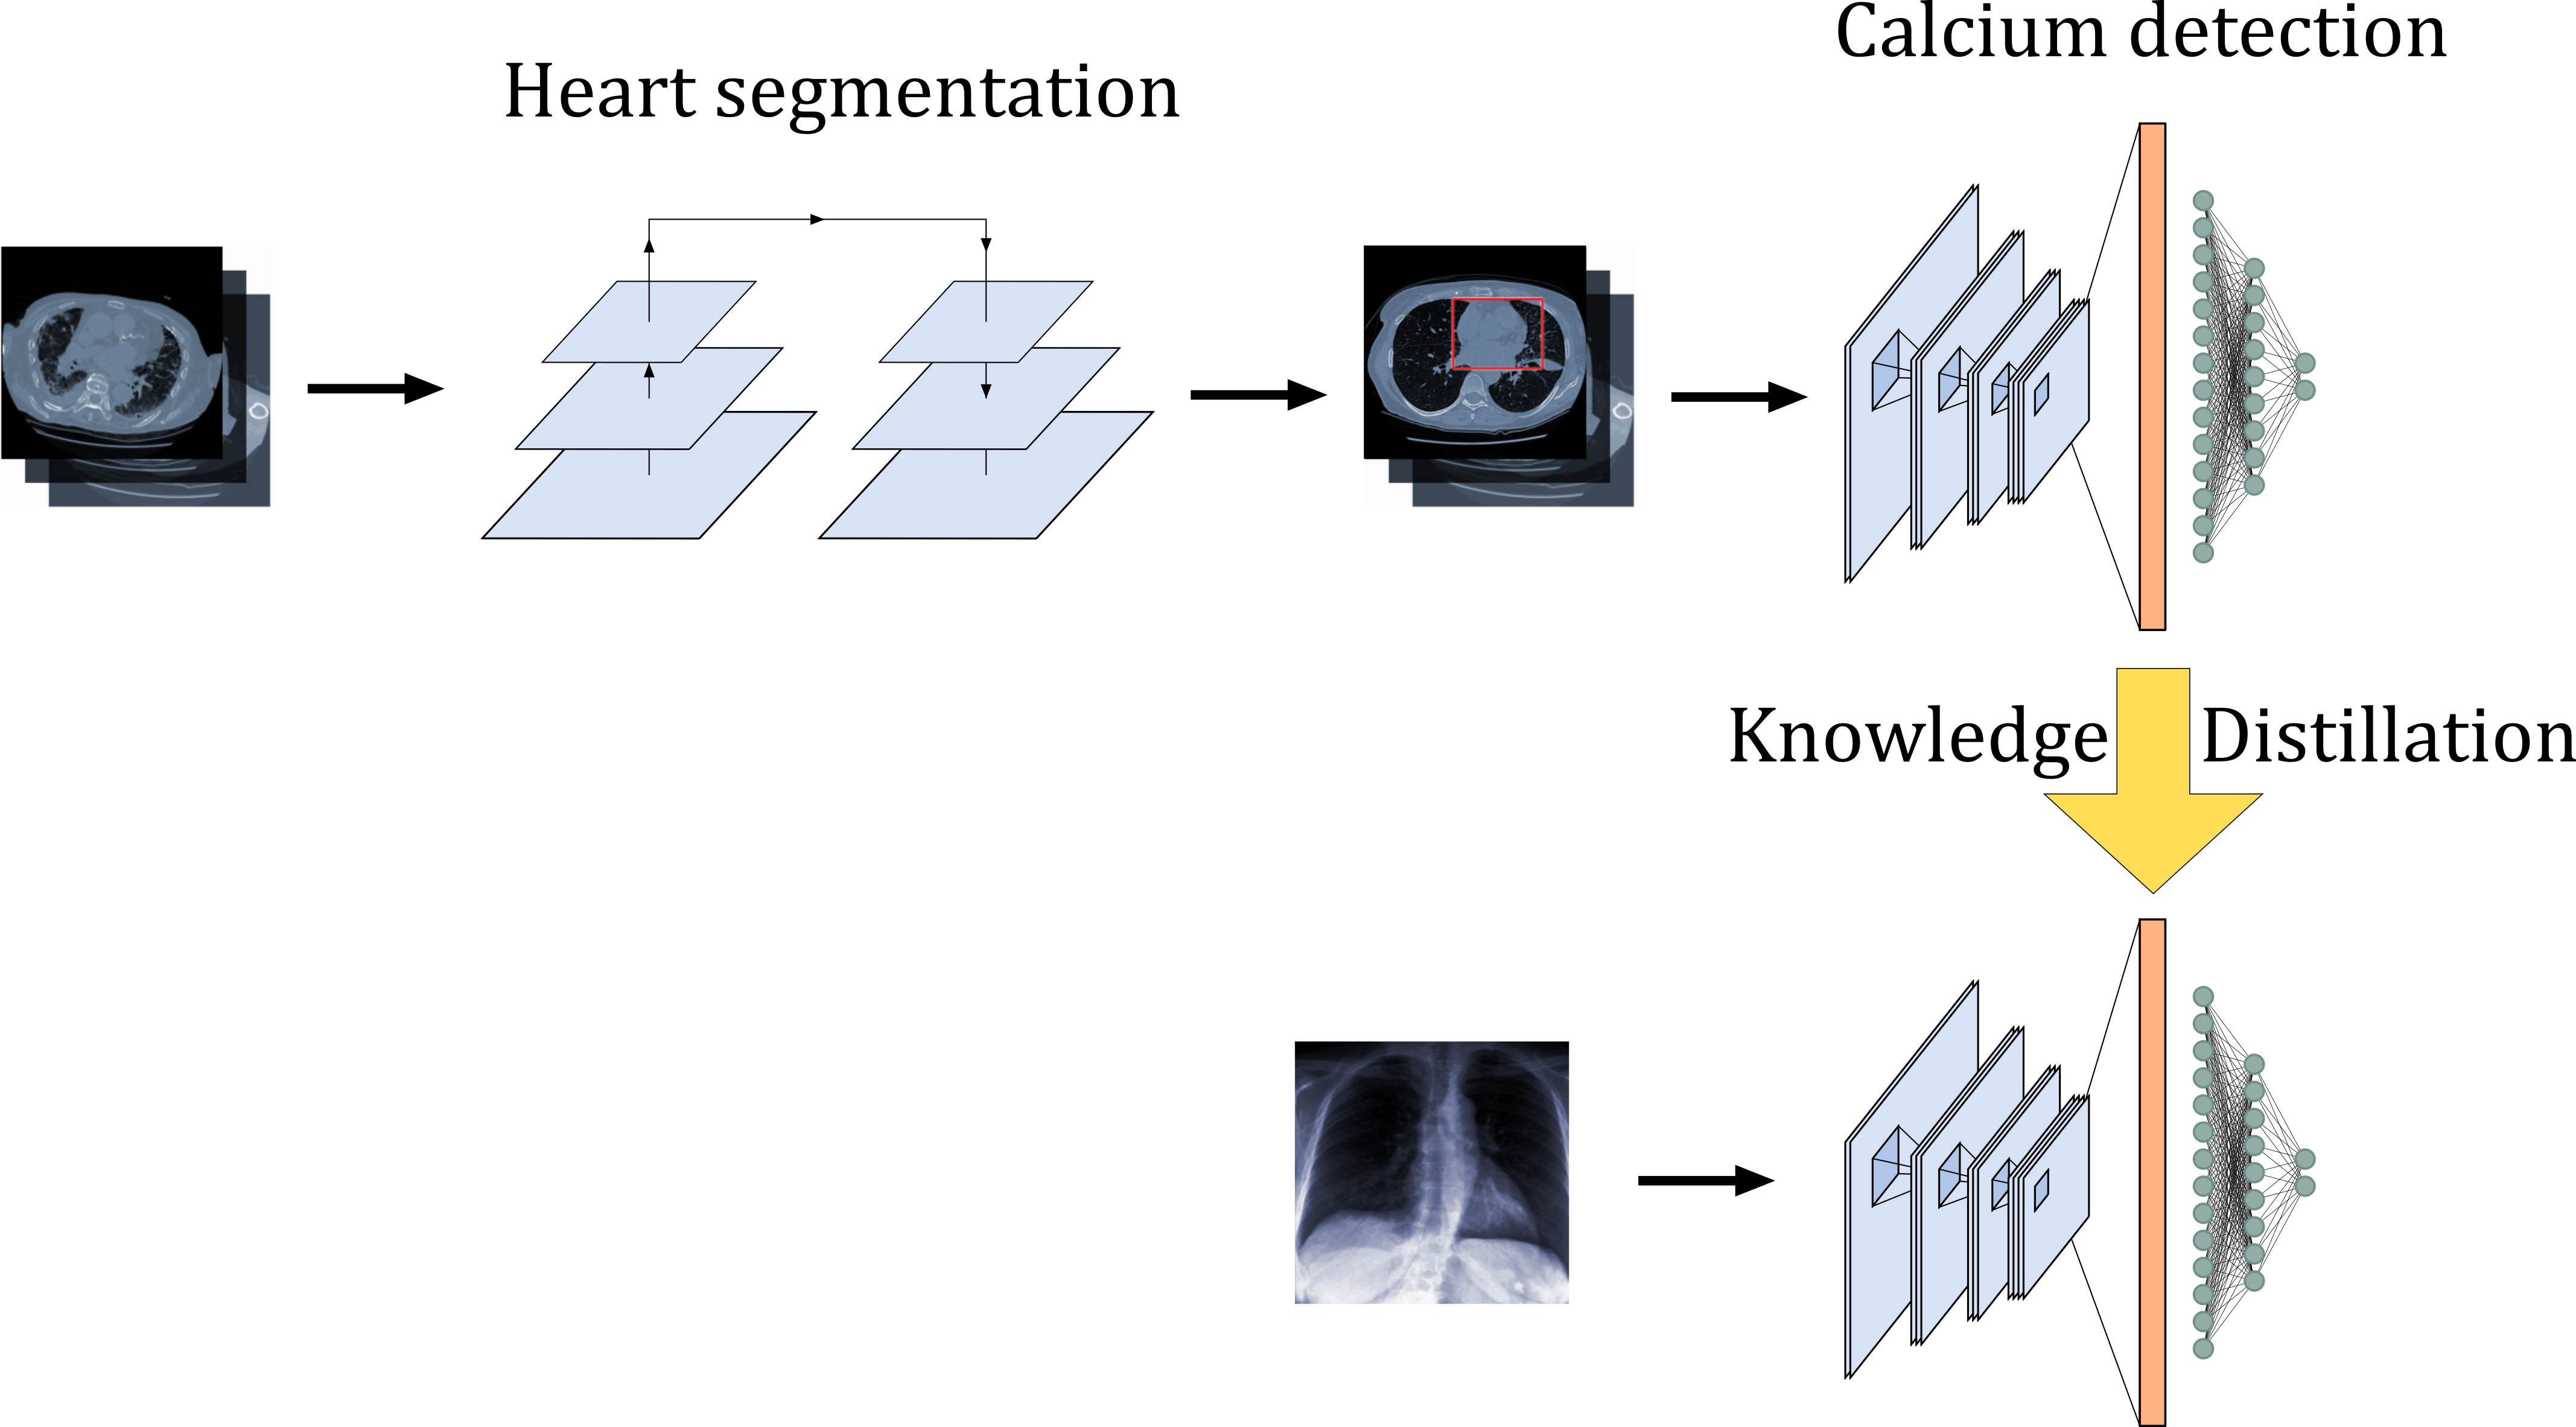
\includegraphics{method} }
    \caption{An overview of the method applied: at first some models are trained on CT scans, then knowledge is distilled from the CT classifier
    to a CXR classifier.}
    \label{fig:method}
\end{figure}

The goal of our work is to train an artificial neural network that can detect if coronary calcium is present or not in a patient from their CXR, to achieve this, we structured the work as a binary classification learning problem.

Due to the inherent complexity of the task and the limited amount of data available, the training has been performed using multi-modal knowledge distillation.
Leveraging peculiarities of our dataset, we used the CT scans to resolve the same classification task, but on a modality in which the problem is actually simpler and already addressed in many works in literature \cite{vanvelzen2021ai}.
Then we exploited the models trained on CTs as teachers to drive the training of a student network that works on the paired CXRs of the same patients.
Since a network trained for a complex task with limited data will likely suffer of overfitting, the idea is to limit it pushing the student to extract better and more generic feature maps while trying to solve the problem and in the meantime mimic behaviour of the teacher which have better generalization capabilities.

An overview of the method is shown in figure \ref{fig:method}.

The rest of this chapter is composed by two sections: at first in \ref{sec:detecting_calcium_on_ct} all the steps for calcium detection on CT scans are presented, including both data preprocessing and model architecture, then on section \ref{sec:detecting_calcium_on_cxr} we describe all the techniques we implemented for detection on CXRs.


\section{Detecting calcium on CT}\label{sec:detecting_calcium_on_ct}

In the last years many methods have been applied to CAC score estimation exploiting CT scans, for example those proposed by \citeauthor{Wolterink2015-ii} \cite{Wolterink2015-ii}, \citeauthor{Lessmann_2018} \cite{Lessmann_2018}, \citeauthor{Cano-Espinosa2018-gm} \cite{Cano-Espinosa2018-gm} and \citeauthor{de_Vos_2019} \cite{de_Vos_2019}, that have been briefly described in section \ref{sec:related_works}.
The availability of many studies on this topic shows that the problem is well known and many techniques have already been explored, sometimes with very good results: \citeauthor{de_Vos_2019} \cite{de_Vos_2019} for example achieved 93\% accuracy on risk category classification.
Interest in the field is also supported by image analysis challenges on this task, such as the \emph{orCaScore} \cite{wolterink2016evaluation} aiming at benchmarking performance of proposed methods.
Test sets contained in challenges typically provide images acquired with a multitude of diverse devices and protocols proving generalization effectiveness and indicating great potential for application in clinical practice \cite{vanvelzen2021ai}.

Many studies are based on 2D convolutional networks working on a single slice of the CT at a time; this is the case, for example, for methods from \citeauthor{Lessmann_2018} \cite{Lessmann_2018} and \citeauthor{de_Vos_2019} \cite{de_Vos_2019}.
This choice is possible whenever the dataset provides a CAC score label for each slice, meaning that, instead of using each CT scan as a single sample, hundreds of images are available for each patient with a single scan, dramatically increasing the size of the dataset.
On the contrary, due to the characteristics of our dataset that provides a single label for each CT, we propose the usage of 3D CNNs working on the whole CT scan.
This introduces additional challenges due to the smaller number of samples and higher computational requirements compared to 2D convolution approach.
In comparison with methods cited above we shall consider, however, that our problem is limited to a classification learning problem with only two classes: positives, with CAC > 0, and negatives, with CAC = 0; then some of the complexity of using 3D convolutions is already mitigated by the simpler task, whereas computational effort is reduced with preprocessing and crop of images as described in next section.


\subsection{Preprocessing of CT}

In order to level out some of the possible differences in images related to the devices used for acquisition and to the different protocols, that could have a negative impact on training, we applied a common preprocessing to them.
At first all the CT scans has been clipped between -1000 and 1000 HU, thus removing spike values below air or above bones density, and then rescaled in range $[-1; 1]$.

Furthermore, since the size of a CT scan is directly related to the amount of memory and time required for its analysis, we identified a method to reduce their size without affecting the quality of data.
The average size of a CT scan in our dataset is $300\times512\times512$ (depth $\times$ height $\times$ width).
It is a very large size that would easily lead to an explosion of parameters in the model, quickly exceeding memory size of a modern powerful GPU.
Also worth to be considered that most of the volume is not involved in CAC score at all; even on CT scans limited to the cardiac area, only few voxels in the image represent calcium lesions in the coronary arteries.
Remove all areas that surely do not contain information about coronary calcium could help also to avoid that spurious correlations between CAC and unrelated characteristics of other body parts could affect training.
The idea is then to reduce the size of the image removing everything that is not included in the near surrounding of the myocardium.
In the next section we describe the steps applied for heart segmentation and crop of the images.


\subsubsection{Cardiac area extraction}

CT scan segmentation is a field that has received a lot of interest and effort, since is often the first step to deal with in order to resolve more complex tasks.
The main challenge to perform segmentation with NN is to have a wide dataset and, for supervised learning, to have high quality annotations of organs and anatomical structures of the body.

An open dataset for heart segmentation has been found in Kaggle platform \cite{kaggle_heart_dataset}.
The training set of this dataset is composed by more than 2500 slices from 19 patients; for each image a corresponding mask of the heart shape is available.
The test set do not include the annotated masks and was not used, to replace it 4 patients from the train set has been excluded during training.
Due to the characteristic of this dataset the model shall work on 2D slices.

We used a library implemented by \citeauthor{Iakubovskii:2019} \cite{Iakubovskii:2019} to easily load well-known models that are at the state of the art for image segmentation.
Two different models have been compared to perform heart segmentation on Kaggle dataset: U-Net \cite{ronneberger2015u} and FPN \cite{lin2017feature}.
These are very similar models that use multiple convolutional and pooling layers to downsample and extract features, then use again convolutions combined with upsampling layers to build a segmentation mask.
The characteristic of these networks is that the features extracted at each downsampling layer are concatenated with each corresponding upsampling step.
The structures of the networks are depicted in figures \ref{fig:unet} and \ref{fig:fpn}.

\begin{figure}
    \centering
    \resizebox{0.9\textwidth}{!}{ 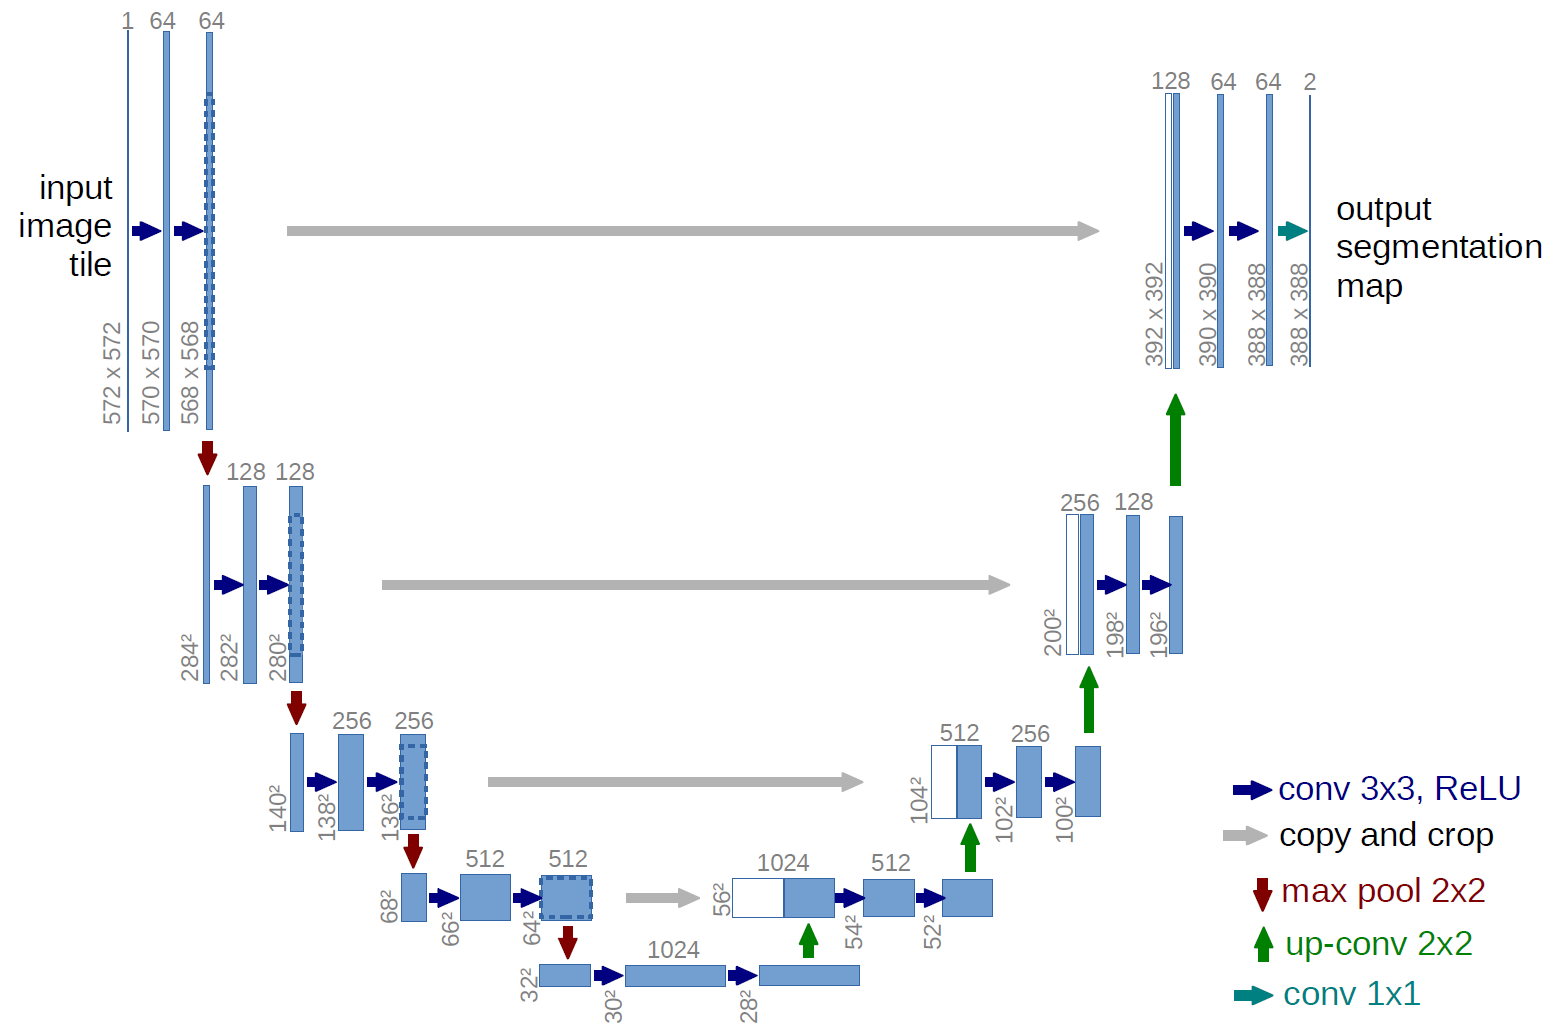
\includegraphics{unet} }
    \caption{U-Net architecture. Image from \cite{ronneberger2015u}}
    \label{fig:unet}
\end{figure}
\begin{figure}
    \centering
    \resizebox{0.6\textwidth}{!}{ 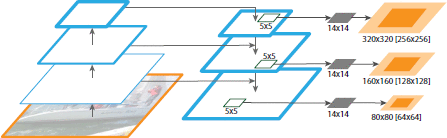
\includegraphics{fpn} }
    \caption{FPN architecture for object segmentation. Image from \cite{lin2017feature}}
    \label{fig:fpn}
\end{figure}

For both models we used a version of the network pre-trained on ImageNet dataset \cite{imagenet_cvpr09} and we evaluated the performance exploiting intersection over union (IoU) score.
Both networks have been trained for 50 epochs on the 15 patients left of the training set.
They achieved very similar results on the test set with a IoU of 0.932 for the U-Net and a IoU of 0.933 for the FPN.
For its slightly better result, predictions from the FPN network were used for the heart crop.

\begin{figure}
    \centering
    \begin{subfigure}[c]{0.3\textwidth}
        \resizebox{\textwidth}{!}{ 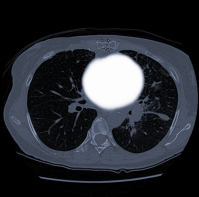
\includegraphics{heart_segmentation_axial} }
        \caption{}
        \label{subfig:heart_segmentation_axial}
    \end{subfigure}\hspace{1em}
    \begin{subfigure}[c]{0.3\textwidth}
        \resizebox{\textwidth}{!}{ 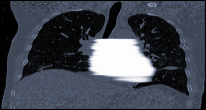
\includegraphics{heart_segmentation_coronal} }
        \caption{}
        \label{subfig:heart_segmentation_coronal}
    \end{subfigure}\hspace{1em}
    \begin{subfigure}[c]{0.3\textwidth}
        \resizebox{\textwidth}{!}{ 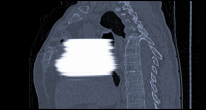
\includegraphics{heart_segmentation_sagittal} }
        \caption{}
        \label{subfig:heart_segmentation_sagittal}
    \end{subfigure}
    
    \caption{Heart segmentation view on (a) axial, (b) coronal and (c) sagittal projections of a CT scan.
             The white area represent the mask predicted by FPN segmentation model.}
    \label{fig:heart_segmentation}
\end{figure}

FPN predictions of heart shape on each slice produce on the CT scan a result that is visible in figure \ref{fig:heart_segmentation}.
The heart seems very well identified even if the areas found by the model are not perfectly aligned on different slices.
To avoid that some false positives distant from the heart could affect the crop, the mask is refined limiting it to the largest connected component only.

A crop of size $150\times220\times280$ is then extracted from the CT scan at the position of the largest connected component found in the mask, downscaling the image to fit the size if required.
The size is determined empirically, with the requirement to fit at least 90\% of the crop areas extracted from our dataset without downscaling. 

For each refined mask, the convex hull including the shape of the heart is calculated using \emph{Quickhull} algorithm \cite{barber1996quickhull}: every voxel out of the hull is then removed setting it to a value of -1000 HU.

The final result of data preparation is shown in figure \ref{fig:heart_crop}.

\begin{figure}
    \centering
    \begin{subfigure}[c]{0.3\textwidth}
        \resizebox{\textwidth}{!}{ 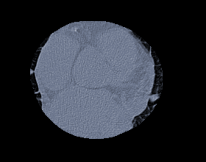
\includegraphics{heart_crop_axial} }
        \caption{}
        \label{subfig:heart_crop_axial}
    \end{subfigure}\hspace{1em}
    \begin{subfigure}[c]{0.3\textwidth}
        \resizebox{\textwidth}{!}{ 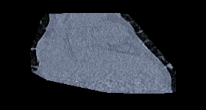
\includegraphics{heart_crop_coronal} }
        \caption{}
        \label{subfig:heart_crop_coronal}
    \end{subfigure}\hspace{1em}
    \begin{subfigure}[c]{0.3\textwidth}
        \resizebox{\textwidth}{!}{ 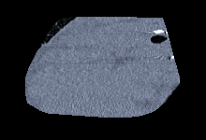
\includegraphics{heart_crop_sagittal} }
        \caption{}
        \label{subfig:heart_crop_sagittal}
    \end{subfigure}
    
    \caption{Final result of data preparation steps view on (a) axial, (b) coronal and (c) sagittal projections of a CT scan.}
    \label{fig:heart_crop}
\end{figure}


\subsection{Architecture of teacher models}

We developed two different models for calcium classification on CT scans.
These are used as teachers in the knowledge distillation training to try to improve performance of CXR classification and therefore is required they perform better than their CXR counterpart.
The two models are built with different structures and complexity in order to verify also impact of model architecture on knowledge distillation; they are:
\begin{enumerate}
    \item \textbf{Simple CT classifier (SimpleCT):} a naive implementation of a CNN with some consecutive convolutional layers followed by a fully
    connected classifier
    \item \textbf{Retina CT classifier (RetinaCT):} a more advanced network derived from RetinaNet \cite{lin2017focal}
\end{enumerate}

In the following paragraphs we detail the characteristics of SimpleCT and RetinaCT, respectively.  


\subsubsection{SimpleCT}
SimpleCT model is composed by 4 convolutional layers followed by an adaptive average pooling and a fully connected classifier.
Each convolutional layer is composed by 3D convolution, ReLU activation, max pooling and batch normalization.
Batch normalization helps to regularize the network and allows to use higher learning rates accelerating training \cite{ioffe2015batch}.
Features extracted by convolutional layers are then flattened by an adaptive average pooling layer that outputs a single average value for each input channel; the flat feature vector is then used to feed a classifier composed by multiple layers of fully connected neurons followed by batch normalization and ReLU activations.
The complete architecture is:

\begin{longtable}{l|l}
    \hline
    \multirow{4}{*}{\textbf{Conv1}} & 3D Convolution (kernel $7\times7\times7$, Stride $2\times2\times1$, 64 out channels) \\
    & ReLU \\
    & Max pooling (kernel $2\times2\times2$) \\
    & Batch normalization \\
    \hline
    \multirow{4}{*}{\textbf{Conv2}} & 3D Convolution (kernel $3\times3\times3$, Stride $1\times1\times1$, 128 out channels) \\
    & ReLU \\
    & Max pooling (kernel $2\times2\times2$) \\
    & Batch normalization \\
    \hline
    \multirow{4}{*}{\textbf{Conv3}} & 3D Convolution (kernel $3\times3\times3$, Stride $1\times1\times1$, 256 out channels) \\
    & ReLU \\
    & Max pooling (kernel $2\times2\times2$) \\
    & Batch normalization \\
    \hline
    \multirow{4}{*}{\textbf{Conv4}} & 3D Convolution (kernel $3\times3\times3$, Stride $1\times1\times1$, 512 out channels) \\
    & ReLU \\
    & Max pooling (kernel $2\times2\times2$) \\
    & Batch normalization \\
    \hline
    \textbf{Adaptavg} & 3D Adaptive average pooling \\
    \hline
    \multirow{3}{*}{\textbf{FC1}} & Linear (512 inputs, 128 outputs) \\
    & Batch normalization \\
    & ReLU \\
    \hline
    \multirow{3}{*}{\textbf{FC2}} & Linear (128 inputs, 32 outputs) \\
    & Batch normalization \\
    & ReLU \\
    \hline
    \textbf{FC3} & Linear (32 inputs, 2 outputs) \\
    \hline
\end{longtable}

\begin{figure}[h]
    \centering
    \resizebox{0.5\textwidth}{!}{ 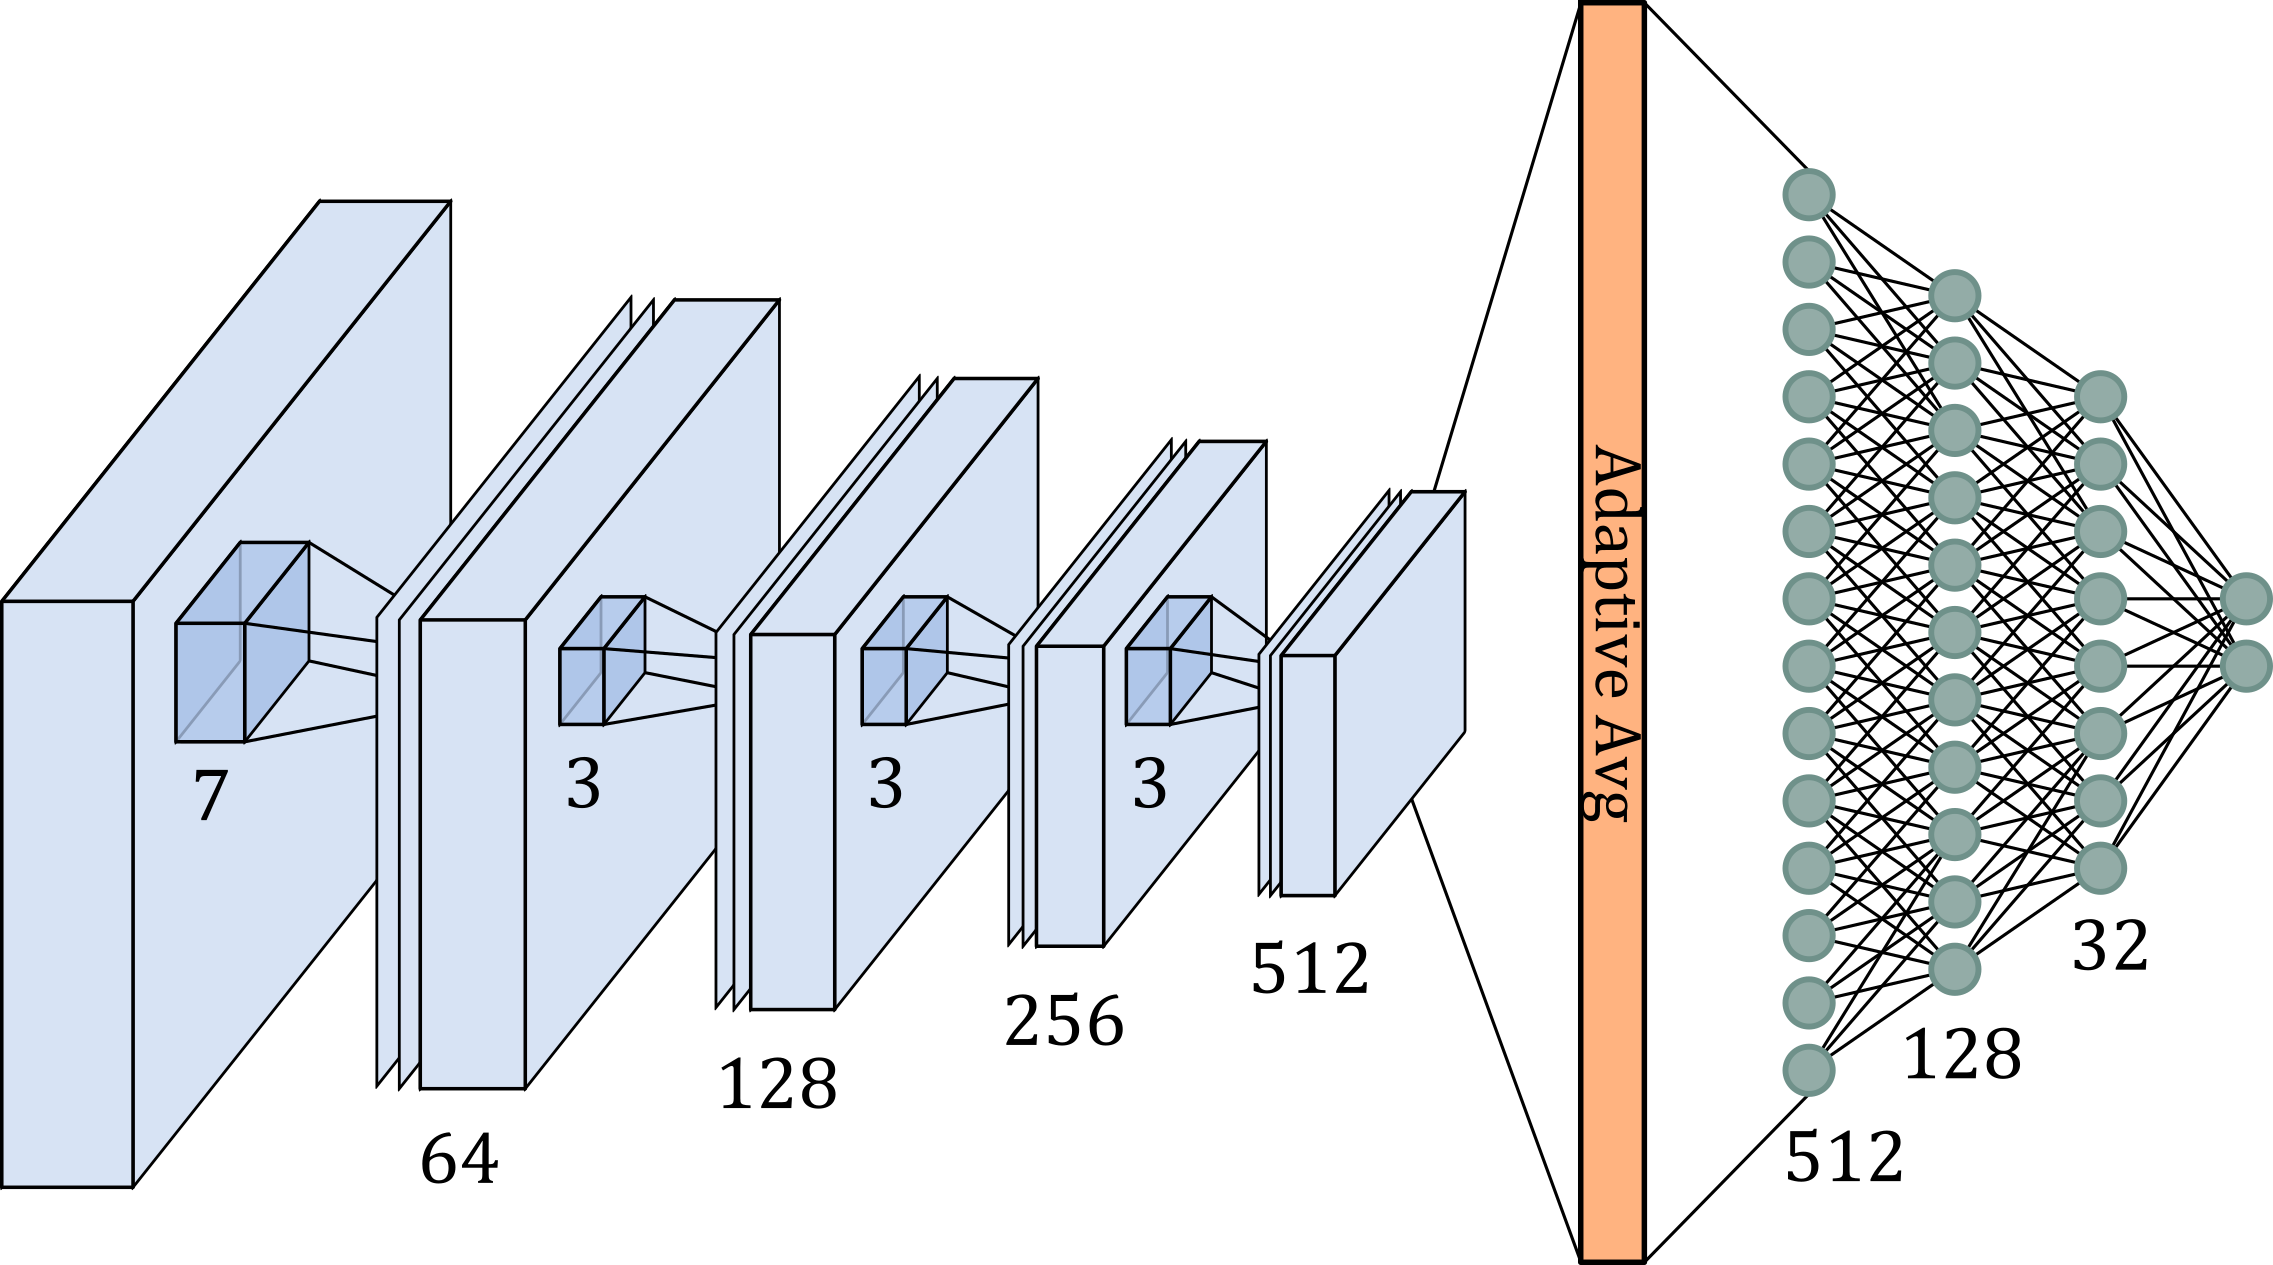
\includegraphics{simple_ct_architecture} }
    \caption{SimpleCT model architecture}
    \label{fig:simple_ct_architecture}
\end{figure}


\subsubsection{RetinaCT}
RetinaCT model is derived from RetinaNet \cite{lin2017focal}, a CNN model for object detection composed by a backbone FPN and two subnets, for object classification and bounding box regression respectively.
In this work we exploited a version of RetinaNet from MonAI project \cite{MONAI} pre-trained on the well-known LUNA16 \cite{luna16} dataset for lung nodules detection. 

From the pre-trained RetinaNet we removed both subnets and the deconvolutional section of the FPN, actually keeping only the basic ResNet \cite{he2016deep} feature extractor.
ResNet is a CNN with additional shortcut connections that add outputs of a convolutional layer to the outputs of a following layer.
The extracted ResNet is then used as the first block of RetinaCT, followed by an adaptive average pooling and a 3-layers fully connected classifier with the same shape as that used in SimpleCT network.

Compared to the previous structure, RetinaCT is more complex, with 23 convolutional layers and shortcut connections, for a total of 2,929,250 training parameters; on the contrary, SimpleCT, despite its simple architecture, is composed by 4,739,874 parameters.

\begin{figure}
    \centering
    \resizebox{0.9\textwidth}{!}{ 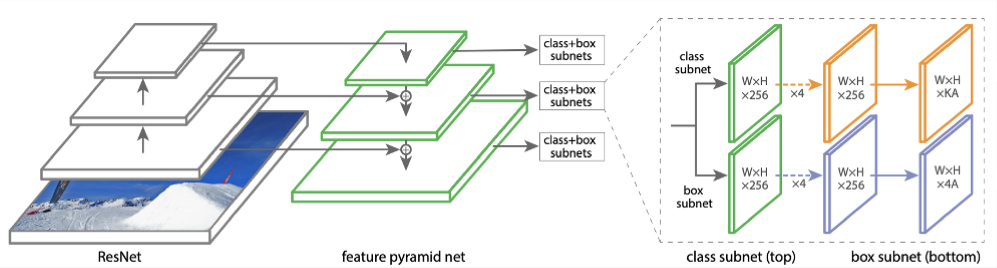
\includegraphics{retinanet_architecture} }
    \caption{RetinaNet architecture. Image from \cite{lin2017focal}}
    \label{fig:retina_net_architecture}
\end{figure}


\subsection{Training on CT}
Both models described in the previous section have been optimized using the cross entropy loss formulated as the equation \ref{eqn:cross_entropy}.
The output logits of the classifier are converted into a probability distribution applying a softmax function formulated as \ref{eqn:softmax}.

Optimization method used is Adam \cite{kingma2014} configured with a learning rate of 0.01, halving it every 20 epochs.

We tried to avoid overfitting by adding also a l2-regularization term to the loss function as follows:
\begin{equation}
    Loss_{l2reg} = Loss(y_i, \hat{y}_i) + \lambda\sum\limits_{i=1}^n w_i^2
    \label{eqn:l2_regularization}
\end{equation}
where $y_i$ and $\hat{y}_i$ are the outputs of the network and the expected results respectively, $w_i$ are the trainable weights of the model, and $\lambda$ is a parameter controlling the importance of the l2 term, which has been set to $10^{-4}$.

In some experiments involving RetinaCT, the first convolutional layers of the pre-trained encoder has been freezed.
This transfer learning approach helps to avoid overfitting that can occur using a high-capacity network as RetinaCT with a small dataset as in our case and can be applied whenever the features extracted are of good quality and source and target domains are similar enough.

Tuning of hyper-parameters has been performed using 5-fold cross validation as reference for evaluation of training performance with special attention to overfitting.
Cross validation has also been used as confirmation of results since our defined test set is quite small and could suffer of undetected biases.
When all parameters are chosen the training is then repeated on the whole training set and generated model performance is finally verified on the test set.


\section{Detecting calcium on CXR}\label{sec:detecting_calcium_on_cxr}

CAC estimation from CXR is considered an hard task if even possible: calcium lesions can be really hard to detect since partially hidden by bones or blended with other tissues due to the 2D projection that is impressed on the X-ray image.
As discussed in section \ref{sec:related_works}, there are very few works trying to estimate CAC score or divides patients on risk categories, with promising results that are, however, still too far from quality required for clinical application.
The contribute of this work is to explore multi-modal knowledge distillation to understand if knowledge learned from CT scans can improve state-of-the-art performance of CAC classification on CXR.
For this purpose we use models described in the previous sections trained on CT scans as teachers to drive training of NNs that use only CXRs as input.


\subsection{Preprocessing of CXR}

We decided to apply to CXRs the same data preprocessing as used in \cite{iodice_2022} since our dataset is an extension of the one used in that work, in order to be able to better compare results.
At first, X-ray images in dicom format are loaded using SimpleITK library \cite{lowekamp2013design} that automatically transforms them to MONOCHROME2 photometric interpretation, if not already in that format: it means that dark areas are used to represent low density tissues, while lighter areas are the high density regions; this is required since some devices generate images using the opposite convention.
Then windowing is applied based on values contained in the metadata.
After that histogram equalization is performed to improve contrast and image is converted to 8 bits per pixel (bpp) to align different resolutions used, varying from 10 to 16 bpp.

Images are then resized to $1248\times1248$ pixels and a center crop of size $1024\times1024$ is extracted.
This crop has been manually verified to not remove any portion of the cardiac area.
Finally pixel values are rescaled in range $[0, 1]$ and normalization of the image is performed, replacing each value $x$ with the formula:
\begin{equation}
    x' = \frac{x - \mu}{\sigma}
    \label{eqn:normalization}
\end{equation}
using $\mu=0.5024$ and $\sigma=0.2898$ calculated as mean and standard deviation of CheXpert dataset, considering it as more representative of radiographs due to its very large size and since some reference models we use are pre-trained on that dataset.


\subsection{Architecture of student model}

The model chosen as the student of the knowledge distillation has a simple architecture, derived directly from SimpleCT model used for classification on CT scans.
The goal is to use a network that is similar enough to the teacher to take advantage of the common structures and easily perform response-based and feature-based KD.

The model is called SimpleCXR and is an adaptation of SimpleCT network replacing each 3D layer with 2D equivalent.
The architecture is then:

\begin{longtable}{l|l}
    \hline
    \multirow{4}{*}{\textbf{Conv1}} & 2D Convolution (kernel $7\times7$, Stride $2\times2$, 64 out channels) \\
    & ReLU \\
    & Max pooling (kernel $2\times2$) \\
    & Batch normalization \\
    \hline
    \multirow{4}{*}{\textbf{Conv2}} & 2D Convolution (kernel $3\times3$, Stride $1\times1$, 128 out channels) \\
    & ReLU \\
    & Max pooling (kernel $2\times2$) \\
    & Batch normalization \\
    \hline
    \multirow{4}{*}{\textbf{Conv3}} & 2D Convolution (kernel $3\times3$, Stride $1\times1$, 256 out channels) \\
    & ReLU \\
    & Max pooling (kernel $2\times2$) \\
    & Batch normalization \\
    \hline
    \multirow{4}{*}{\textbf{Conv4}} & 2D Convolution (kernel $3\times3$, Stride $1\times1$, 512 out channels) \\
    & ReLU \\
    & Max pooling (kernel $2\times2$) \\
    & Batch normalization \\
    \hline
    \textbf{Adaptavg} & 2D Adaptive average pooling \\
    \hline
    \multirow{3}{*}{\textbf{FC1}} & Linear (512 inputs, 128 outputs) \\
    & Batch normalization \\
    & ReLU \\
    \hline
    \multirow{3}{*}{\textbf{FC2}} & Linear (128 inputs, 32 outputs) \\
    & Batch normalization \\
    & ReLU \\
    \hline
    \textbf{FC3} & Linear (32 inputs, 2 outputs) \\
    \hline
\end{longtable}


\subsection{Training on CXR using KD}\label{sec:training_on_cxr}

Training is performed by adding a knowledge distillation term on the usual loss function.
The optimized loss is then a combination of two functions:
\begin{equation}
    \mathcal{L} = (1 - \alpha_{KD})\mathcal{L}_{GT} + \alpha_{KD}\mathcal{L}_{KD}
    \label{eqn:kd_loss}
\end{equation}
where $\mathcal{L}_{GT}$ is the cross-entropy loss calculated on hard targets, i.e. the ground truth labels, $\mathcal{L}_{KD}$ is the KD loss and $\alpha_{KD}$ is a parameter used to adjust the importance of KD.

The KD applied is always multi-modal, using networks trained on CTs as teacher.
Teachers are all pre-trained and freezed during distillation, using the so-called offline approach.

We tested two different ways to distill knowledge, namely response-based and feature-based.
In response-based knowledge approach we compare the output logits of both teacher and student models, at first converting them to probability distributions using the softmax function as defined in \ref{eqn:softmax} and then calculating their distance using the the Kullback-Leibler divergence as formulated in \ref{eqn:kldiv}.
This distance is used as the $\mathcal{L}_{KD}$ term of the loss function.
Formulation of this term can then be written as:
\begin{equation}
    L_{ResD}(\hat{z}, z, T) = \sum_{i=1}^{N} p(\hat{z}_i, T) log\frac{p(\hat{z}_i, T)}{p(z_i, T)}
    \label{eqn:resp_kd_loss}
\end{equation}
where $\hat{z}$ and $z$ are respectively the teacher and the student logits, $p$ is the softmax function and $T$ is the temperature term, used to soften probability distribution over classes $i$.

For the feature-based knowledge, instead, we chose some internal feature layers of both teacher and student to compare, using MSE as formulated in \ref{eqn:mse} as loss.
The $\mathcal{L}_{KD}$ term in this case is:
\begin{equation}
    L_{FeaD}(\hat{f}, f) = \frac{1}{n} \sum\limits_{i=1}^n (f_i - \hat{f}_i)^2
    \label{eqn:feat_kd_loss}
\end{equation}
where $\hat{f}$ and $f$ are the feature maps extracted by teacher and student respectively.

We experimented two different approaches of feature-based distillation, the former compare the outputs of the last layer of the encoders of both models; the latter uses a separate branch composed by two fully-connected layers attached to the encoder of the student network, and compare the output of this projection head to an internal feature map extracted by an intermediate layer of the teacher classifier.
This strategy relaxes the requirement for the student to have an internal feature map matching exactly a feature map of the teacher, to the requirement to have the same informative content that can be transformed in some way to match the teacher.
The idea is borrowed from a work by \citeauthor{fini2022self} \cite{fini2022self} where distillation was not performed between the outputs of the two networks but a branch was added to the student.

The training architecture for feature-based knowledge using a separate branch is shown in figure \ref{fig:feature_based_branch_kd}.

\begin{figure}
    \centering
    \resizebox{\textwidth}{!}{ 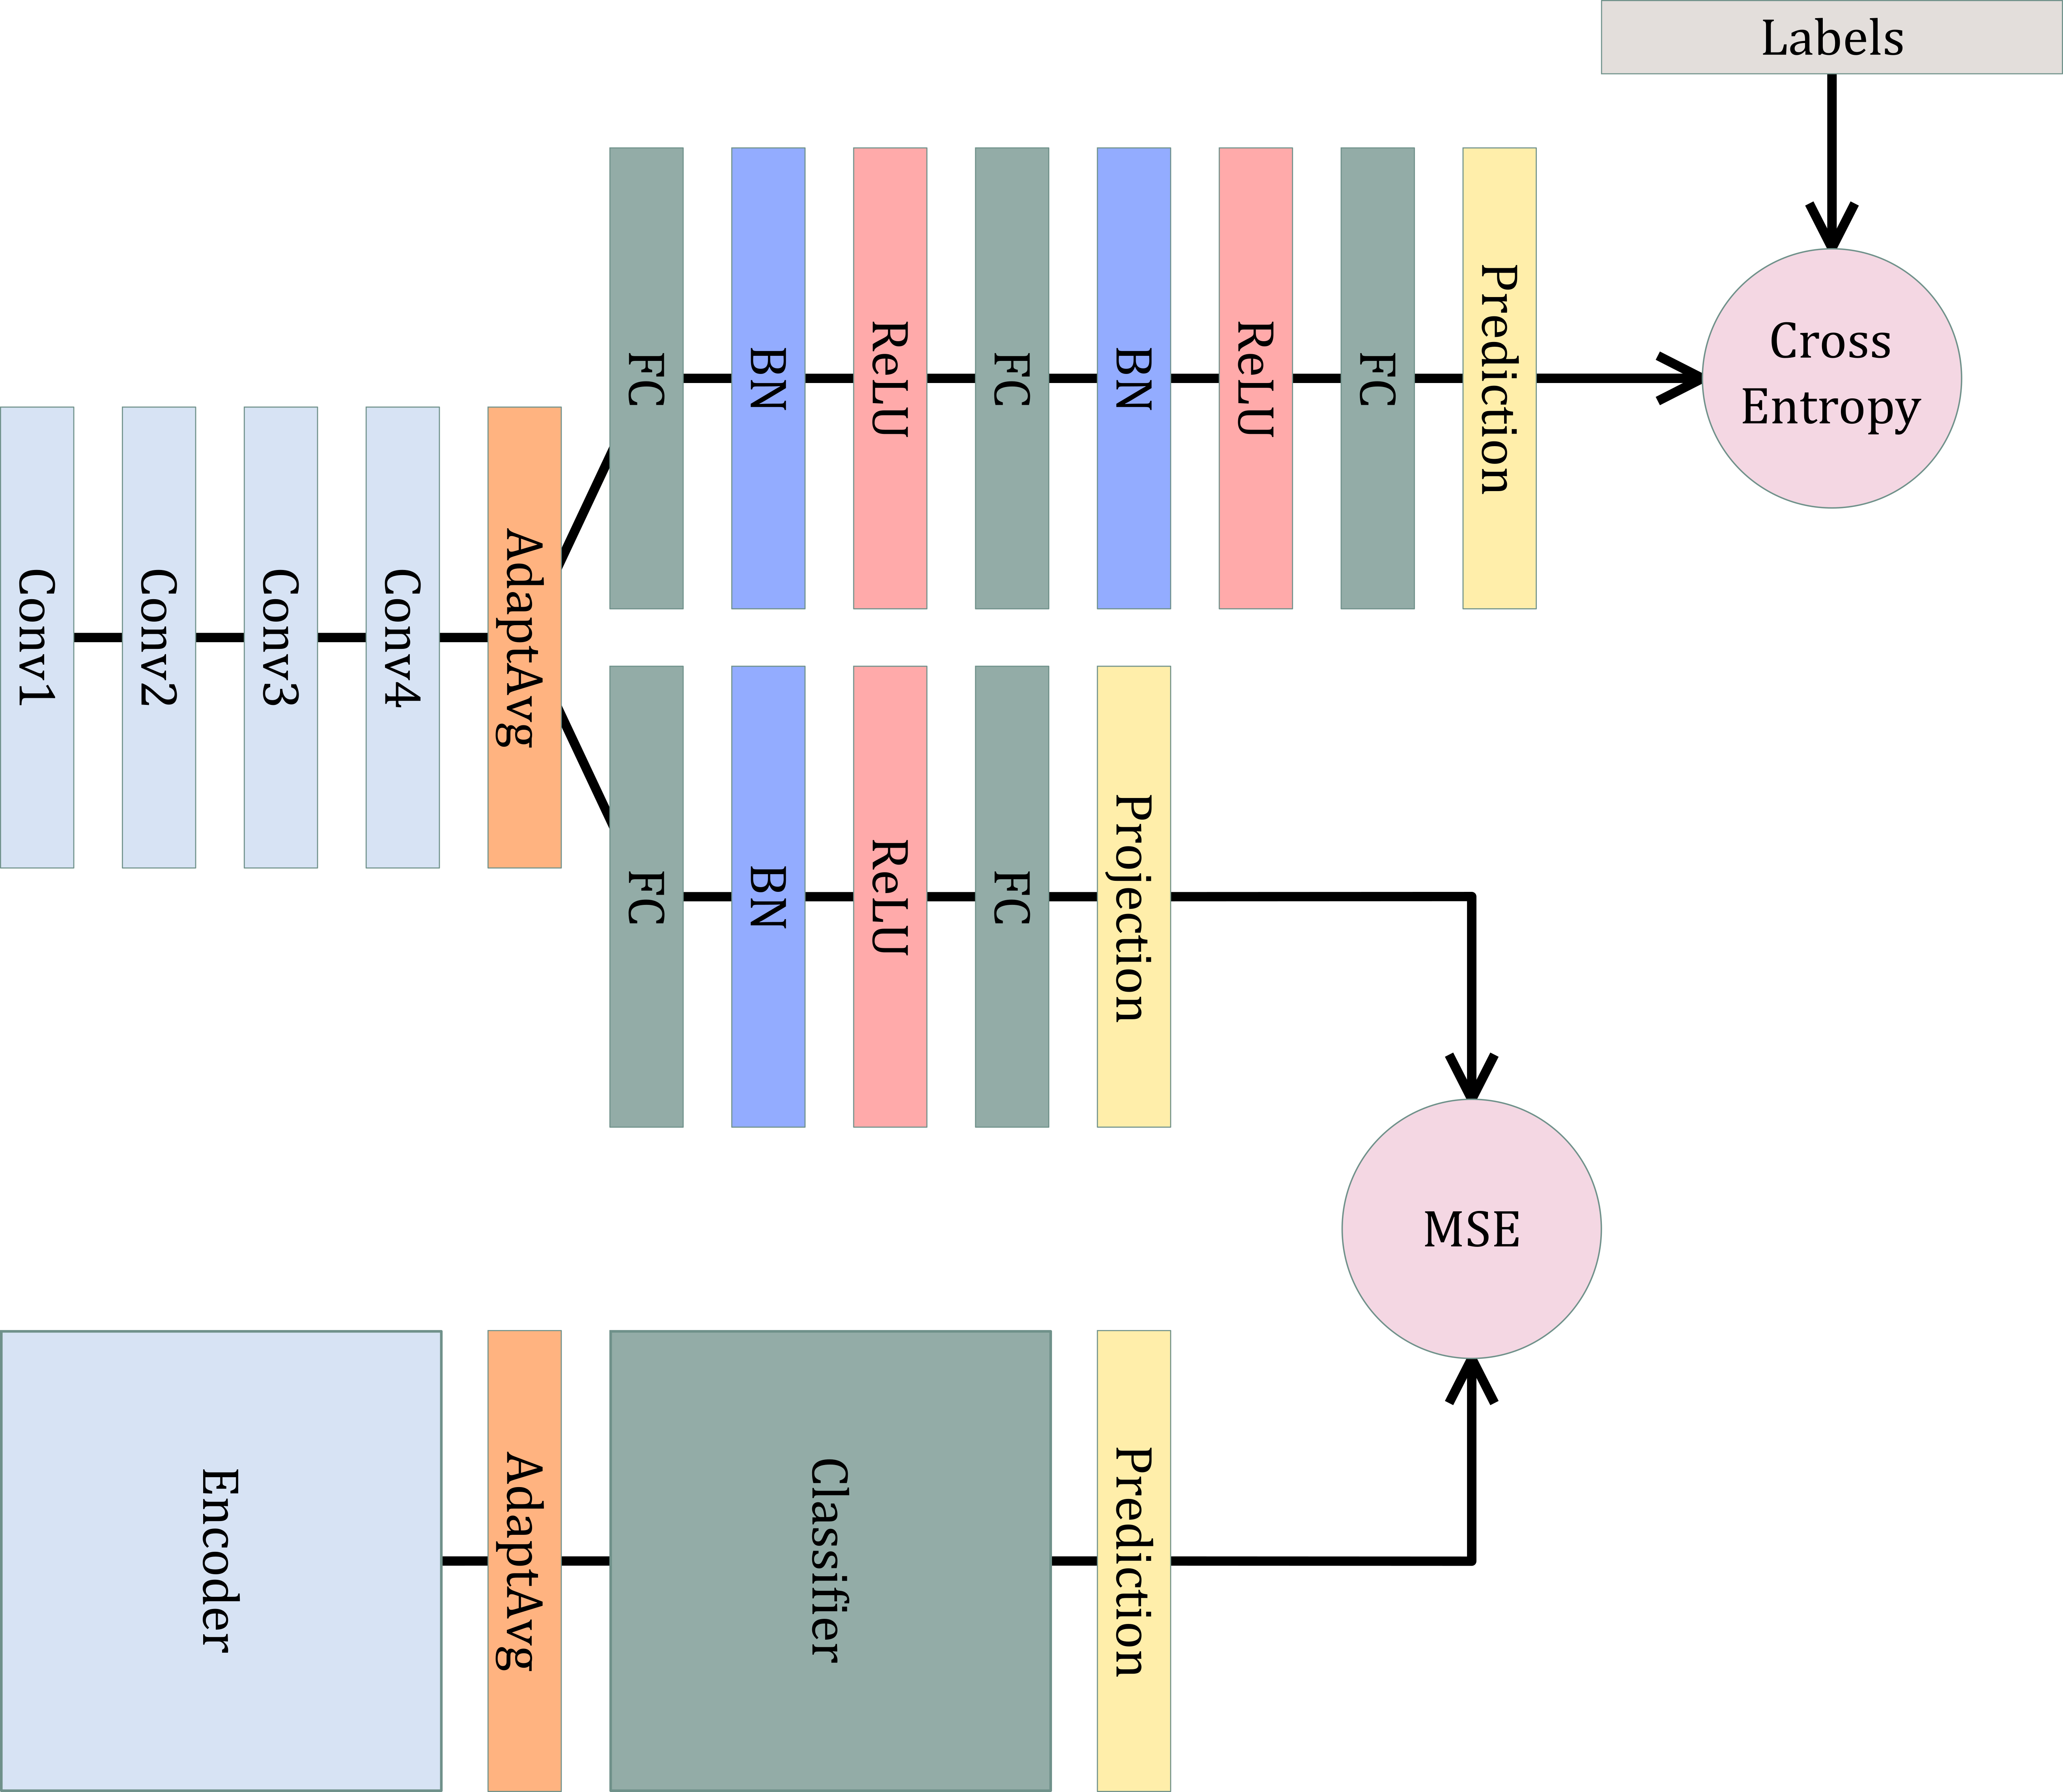
\includegraphics{feature_based_kd} }
    \caption{Architecture of feature-based knowledge distillation method using a separate branch}
    \label{fig:feature_based_branch_kd}
\end{figure}

Regardless of the distillation strategy used, the optimization method is always Adam with learning rate set to 0.005.
Learning rate decay is applied and also l2-regularization is used in some experiments.


\subsection{Baseline methods using CXR only}

To have a reference for comparison of results with those obtained using knowledge distillation approach, we trained other two models.

At first we trained \emph{SimpleCXR} using CXR images only.
Training is performed for 200 epochs with a batch size of 4 samples, optimized using Adam with a learning rate of 0.005 using decay and l2-regularization.
This approach is deliberately very similar to that applied to training with knowledge distillation, except for the KD term that is not present here, and is used as reference to verify if KD is beneficial to improve performance of \emph{SimpleCXR} network on our task.

The second model we used as baseline, is trained using the best configuration found on Iodice masters' thesis \cite{iodice_2022} which obtained, up to our knowledge, the best results for classification on this dataset and on this task in general.

The model is based on a DenseNet-121 \cite{huang2018densely}, that is a very deep CNN on which, similarly to ResNet, some shortcut connections are added, but in this case the outputs of each convolutional layer in a block are concatenated instead of added to outputs of all following one; in this way each layer receives the feature maps of all preceding layers.
Between dense blocks a transition layer is placed that performs downscale with pooling.
An example of DenseNet with 3 dense blocks is shown in figure \ref{fig:densenet}.

\begin{figure}
    \centering
    \resizebox{\textwidth}{!}{ 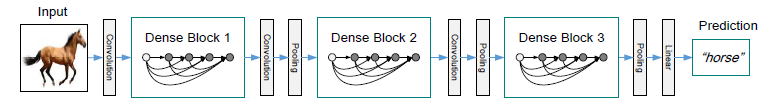
\includegraphics{densenet} }
    \caption{A DenseNet with 3 dense block. Image from \cite{huang2018densely}}
    \label{fig:densenet}
\end{figure}

The model encoder is pre-trained on CheXpert dataset and the original hierarchical classifier is replaced with a 2-layers classifier.
The complete architecture is thus as follows:

\vspace{1em}
\begin{tabular}{l|cl}
    \hline
    \multirow{7}{*}{\begin{minipage}{7em}\textbf{DenseNet-121 encoder}\end{minipage}}
    & \freeze & Dense block (6 dense layers, 256 out channels) \\
    & \freeze & Transition layer (128 out channels) \\
    & \freeze & Dense block (12 dense layers, 512 out channels) \\
    & \freeze & Transition layer (256 out channels) \\
    & \freeze & Dense block (24 dense layers, 1024 out channels) \\
    & \freeze & Transition layer (512 out channels) \\
    & & Dense block (16 dense layers, 1024 out channels) \\
    \hline
    \textbf{Adaptavg} & & Adaptive average pooling \\
    \hline
    \multirow{3}{*}{\textbf{Classifier}} & & Linear (1024 inputs, 64 outputs) \\
    & & ReLU \\
    & & Linear (64 inputs, 2 outputs) \\
    \hline
\end{tabular}
\vspace{1em}

The total number of training parameters in the network is 7,013,314.
Most of them, up to the last convolutional layer of the last dense block, are actually freezed during training on calcium dataset.

We used AdamW as optimizer, an implementation of Adam contained in pytorch library \cite{pytorch}, with a learning rate of 0.003 that is decayed at step 20 and 35, multiplying the value for a factor of 0.1.
L2-regularization is also applied with $\lambda$ parameter set to $10^{-4}$.
Training is performed for 50 epochs with a batch size of 4 samples.
Results are evaluated using 5-fold cross validation.
